% rubber: setlist arguments --shell-escape
\documentclass[final,t]{beamer}
\mode<presentation>{\usetheme{I6dv}}
\setbeamerfont{itemize}{size=\normalsize}
\setbeamerfont{itemize/enumerate body}{size=\normalsize}
\setbeamerfont{itemize/enumerate subbody}{size=\normalsize}
\usepackage{amsmath,amsthm,amssymb,latexsym}
\usepackage{minted, verbatim}
\usepackage[english]{babel}
\usepackage[latin1]{inputenc}
\usepackage[orientation=landscape,size=custom,width=200,height=120,scale=1.9]{beamerposter}

\title{\huge Visualizing Parallelism in CS 2: Report from a Spring 2012 Early
Adopter}
\author[Sean Massung and Cinda Heeren]{Sean Massung and Cinda Heeren,
\texttt{\{massung1,c-heeren\}@illinois.edu}}
\institute[University of Illinois]{University of Illinois at Urbana-Champaign,
College of Engineering, Department of Computer Science}
\date{}

\newminted{cpp}{fontsize=\small}

\begin{document}
\begin{frame}[fragile]{}
    \begin{columns}[t]
        \begin{column}{.3\linewidth}
            \begin{block}{Introduction}
                \begin{itemize}
                    \item We describe the incorporation of the IEEE-TCPP
                        Curriculum Initiative into CS 2 at the University of
                        Illinois
                    \item We focus on three main parallel programming concepts,
                        each delivered during a two hour discussion/lab section.
                        Material from these lab sections is graded, and some key
                        topics are evaluated on exams in the form of multiple
                        choice questions.
                    \item The three lessons explore the basics of parallelism in a
                        \alert{visual} manner: using OpenMP, race conditions,
                        and reductions
                    \item Tethering images to understanding parallelism enhances
                        student interest and provides an alternative route to
                        mastery of the material.
                    \item Parallelizing an operation across image partitions is
                        much more intriguing than divvying up rows and columns
                        in a matrix!
                \end{itemize}
            \end{block}
            \begin{block}{Lab 1: Intro to Parallelism}
                \begin{itemize}
                    \item In the coding portion of the lab, we expose students
                        to computation across threads.
                    \item For one task, students simply write a function that
                        removes the green color component from an image.
                \end{itemize}
                \begin{cppcode}
#pragma omp parallel for
for(int i = 0; i < width; ++i) {
   for(int j = 0; j < height; ++j) {
      *output(i, j) = *source(i, j);
       output(i, j)->green = 0;
   }
}
                \end{cppcode}
                \begin{itemize}
                \item To illustrate the progress of the parallelized code we
                    give the students augmented code that stops execution midway
                    through the operation
                \item They see that there are four threads operating on the
                    image removing the green component
                \item The threads are partitioning the image along the width as
                    shown in the code snippet; each thread operates on one fourth of the
                    image
                \end{itemize}
                \vspace*{1.0in}
                \begin{tabular}{cc}
                \includegraphics[width=11.0in]{semi-processed-remove.png}
                &
                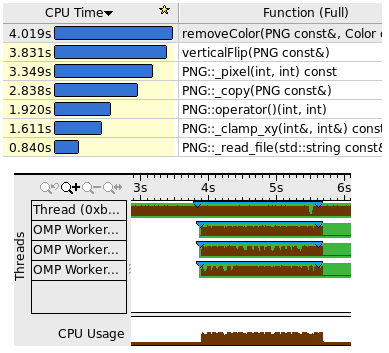
\includegraphics[width=7.5in]{tool-small.png}
                \\
                \emph{Removing a color} &
                \emph{Visualization of threads} \\
                \end{tabular}
                \vspace*{1.0in}
                \begin{itemize}
                    \item Students parallel profiling tools to profile the
                        execution of serial code
                    \item They  select the two most time-expensive functions to
                        parallelize, and speculate on expected speedup under
                        parallel computation \emph{a la} Amdahl's Law
                    \item The profiler's processor usage charts are particularly
                        informative over simple metrics like overall CPU
                        consumption. Since these graphs show thread usage over
                        time, the students can see which portions of their
                        programs run efficiently in parallel
                \end{itemize}
                \vspace*{1.2in}
            \end{block}
        \end{column}
        \begin{column}{.3\linewidth}
            \begin{block}{Lab 2: Race Conditions}
                \begin{itemize}
                    \item Race conditions are the main topic in the second lab
                        section. Students learn that correctly parallelizing
                        programs does not just consist of blindly pasting a
                        \verb|#pragma| on an outer for loop. An incorrect
                        parallel image flipper is below:
                \end{itemize}
                \begin{cppcode}
RGBAPixel temp;
#pragma omp parallel for
for(int i = 0; i < width; ++i) {
   for(int j = 0; j < height / 2; ++j) {
      temp = *image(i, j);
      *image(i, j) = *image(i, height - 1 - j);
      *image(i, height - 1 - j) = temp;
   }
}
                \end{cppcode}
                \begin{tabular}{cc}
                    \includegraphics[width=11.0in]{flipped.png}
                &
                \begin{minipage}[b]{.5\textwidth}
                    \begin{itemize}
                        \item Moving the declaration \verb|RGBAPixel temp|
                            inside the for loop fixes the problem, creating a
                            local \verb|temp| variable for each thread (that
                            does not get clobbered)
                        \item We introduce \verb|#pragma omp critical|, which
                        allows only one thread to operate on the critical
                        section of code at one time. We explain how critical
                        regions are a possible solution to some race conditions 
                    \end{itemize}
                \end{minipage} \\
            \end{tabular}
            \end{block}
            \begin{block}{Lab 3: Reductions}
                \begin{itemize}
                    \item The last lab section introduces a paradigm for
                        solving complex data dependency issues, namely {\em
                        reductions}.  We present reductions as a general
                        algorithmic technique, so as to  provide a stepping
                        stone to understanding the MapReduce programming
                        model
                \end{itemize}
                \begin{cppcode}
map<RGBAPixel, int> ret_freq;
#pragma omp parallel
{
   map<RGBAPixel, int> local_freq;
#pragma omp for
   for(int i = 0; i < width; ++i) {
      for(int j = 0; j < height; ++j)
          ++local_freq[ *image(i,j) ];
   }
#pragma omp critical
   {
       map<RGBAPixel, int>::iterator curr = local_freq.begin();
      for( ; curr != local_freq.end(); ++curr) {
         int count = curr->second;
         ret_freq[ curr->first ] += count;
      }
   }
}
return ret_freq;
                \end{cppcode}
                \begin{tabular}{cc}
                    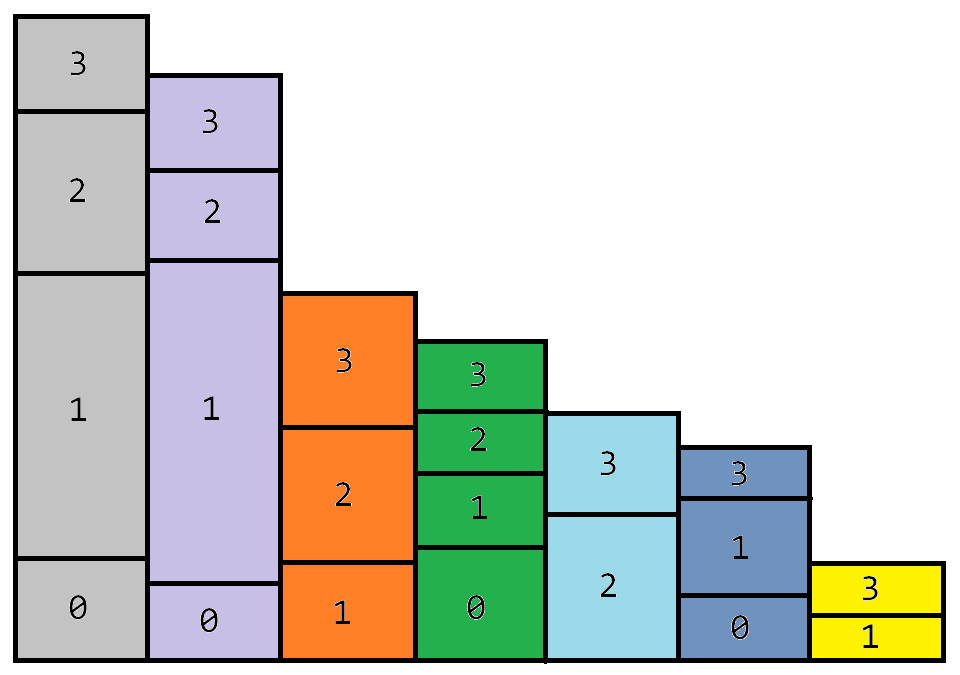
\includegraphics[width=8.0in]{chart.png}
                &
                \begin{minipage}[b]{.6\textwidth}
                    \begin{itemize}
                        \item We ask students to create a PNG color histogram.
                            To do so we simply record the number of pixels of
                            each color.  This is trivial in serial, but requires
                            a slightly different approach when applied across
                            many threads, since the sub-problems on each thread
                            must be combined into the whole
                        \item Provided code creates a histogram of colors,
                            broken down by which thread counted them (0 to 3)
                    \end{itemize}
                \end{minipage} \\
            \end{tabular}
            \end{block}
        \end{column}
        \begin{column}{.3\linewidth}
            \begin{block}{Evaluation}

                \begin{itemize}
                    \item
                    Student performance on lab exercises was exemplary with
                    average scores of 95\% on all three assignments.  Besides
                    grading lab work, questions regarding parallelism were
                    included on exams. Below are examples of the questions we
                    have assessed on various tests over the past two semesters.

                    \item
                    The first asks students to diagnose data races in small
                    sections of parallel code.

                \end{itemize}

                \begin{cppcode}
// (i)
#pragma omp parallel for
for (int i = 1; i < 100; i++)
    colorArray[i] = colorArray[i-1];
// (ii)
#pragma omp parallel for
for (int i = 0; i < width; i++) {
    for (int j = 0; j < height/2; j++) {
        RGBAPixel temp = *img(i, j);
        *img(i,j) = *img(i, height-1-j);
        *img(i, height-1-j) = temp;
    }
}
// (iii)    
#pragma omp parallel for
for(int i = 0; i < 10; i++)
    for(int j = 0; j < 10; j++)
        table[i][j] = (i+1)*(j+1); 
                \end{cppcode}

                Which of the code examples above is/are NOT correctly parallelized?

                \begin{enumerate}[(a)]
                    \setlength\itemindent{2cm}
                    \item Only item (i) is incorrect.
                    \item Only item (ii) is incorrect.
                    \item Only item (iii) is incorrect.
                    \item Two of the above examples are incorrect.
                    \item All statements (i), (ii), and (iii) are correct.
                \end{enumerate}
~ \\
~ \\
                Another typical question simply tests knowledge of the term
                    \emph{reduction}, and its use in a parallel context.  Again,
                    student performance is not nearly perfect--typically only 50
                    to 60\% of students answer correctly.
                \begin{tabular}{p{10in}p{10in}}
                    What is the best definition of the term \emph{reduction}?
                    \begin{enumerate}
                        \setlength\itemindent{2cm}
                        \item A reduction performs the same instructions on data
                            across multiple threads.
                        \item A reduction occurs when private data on individual
                            threads is assembled into a general solution.
                        \item Reduction is a technique wherein parallelism is
                            applied to the portion of a program that requires
                            the most computation. 
                        \item Reduction is just another term for {\em speedup}.
                        \item None of these is the correct choice.
                    \end{enumerate}
                    &  
                    Suppose an algorithm takes 7 seconds to run serially, and 2 seconds to run in parallel.  Then the {\em speedup} for the parallelized code is:
                    \begin{enumerate}
                        \setlength\itemindent{2cm}
                        \item $\frac{2}{7}$
                        \item $\frac{7}{2}$
                        \item $\frac{7-2}{7}$
                        \item The speedup cannot be determined because the number of processors is not known.
                        \item None of these answers is correct.
                \end{enumerate} \\
                \end{tabular}
                \vspace*{2.0in}
            \end{block}
        \end{column}
    \end{columns}
\end{frame}
\end{document}
